\documentclass[12pt,letterpaper]{article}
\usepackage[utf8]{inputenc}
\usepackage[spanish]{babel}
\usepackage{graphicx}
\usepackage[left=2cm,right=2cm,top=2cm,bottom=2cm]{geometry}
\usepackage{graphicx} % figuras
% \usepackage{subfigure} % subfiguras
\usepackage{float} % para usar [H]
\usepackage{amsmath}
%\usepackage{txfonts}
\usepackage{stackrel} 
\usepackage{multirow}
\usepackage{enumerate} % enumerados
\renewcommand{\labelitemi}{$-$}
\renewcommand{\labelitemii}{$\cdot$}
% \author{}
% \title{Caratula}
\begin{document}

% Fancy Header and Footer
% \usepackage{fancyhdr}
% \pagestyle{fancy}
% \cfoot{}
% \rfoot{\thepage}
%

% \usepackage[hidelinks]{hyperref} % CREA HYPERVINCULOS EN INDICE

% \author{}
\title{Caratula}

\begin{titlepage}
\begin{center}
\large{UNIVERSIDAD PRIVADA DE TACNA}\\
\vspace*{-0.025in}
\begin{figure}[htb]
\begin{center}

\includegraphics[width=4cm]{./images/logo}
\end{center}
\end{figure}
\vspace*{0.15in}
INGENIERIA DE SISTEMAS  \\

\vspace*{0.5in}
\begin{large}
TEMA:\\
\end{large}

\vspace*{0.1in}
\begin{Large}
\textbf{Patrones de Diseño Arquitecturales y Estructurales} \\
\end{Large}

\vspace*{0.3in}
\begin{Large}
\textbf{CURSO:} \\
\end{Large}

\vspace*{0.1in}
\begin{large}
BASE DE DATOS II\\
\end{large}

\vspace*{0.3in}
\begin{Large}
\textbf{DOCENTE(ING):} \\
\end{Large}

\vspace*{0.1in}
\begin{large}
 Patrick Jose Cuadros Quiroga\\
\end{large}

\vspace*{0.2in}
\vspace*{0.1in}
\begin{large}
Integrantes: \\
\begin{flushleft}
Andree Ludwed VELASCO SUCAPUCA	\hfill	(20161515) \\
Yofer Nain CATARI CABRERA		\hfill	(2017059289) \\
Marko Antonio RIVAS RIOS          	\hfill	(2016055461) \\
Jorge Luis MAMANI MAQUERA    	\hfill	(2016055236) \\
Jesus ESCALANTE ALANOCA   	\hfill	(2015050641) \\
Adnner Sleyder ESPERILLA RUIZ		\hfill	(2015050543) \\
\end{flushleft}
\end{large}
\end{center}

\end{titlepage}


\tableofcontents % INDICE
\thispagestyle{empty} % INDICE SIN NUMERO
\newpage
\setcounter{page}{1} % REINICIAR CONTADOR DE PAGINAS DESPUES DEL INDICE

\section{ Introducción} 
\textbf{¿Cómo surgen los patrones de diseño?}\\
\begin{flushleft}
Los patrones de diseño son la base para la búsqueda de soluciones a problemas comunes en el desarrollo de software y otros ámbitos referentes al diseño de interacción o interfaces.
Un patrón de diseño resulta ser una solución a un problema de diseño.
\end{flushleft}

\section{ Arquitectura de Software basada en unModelo de Capas para Entornos de CC} 
\textbf{........................................}\\
\begin{flushleft}
......................................
\end{flushleft}
\section{ Patrones Arquitectónicosl} 
\textbf{........................................}\\
\begin{flushleft}
......................................
\end{flushleft}
\section{Patrones de Diseño (Facade)} 
\textbf{}\\
\begin{flushleft}
Los patrones de diseño se consideran una de las herramientas más valiosas para producir diseños de calidad y una técnica de propósito general para mejorar un diseño es identificar todas las realizaciones de patrones y aplicar reglas conocidas para mejorarlos.

\begin{itemize}
	\item Patrones de Diseño
	\\IDEA es un asistente de diseño interactivo para arquitectos de software destinado a automatizar la tarea de encontrar y mejorar las realizaciones de los patrones de diseño.


	


	\item ¿Qué es una fachada o facade en inglés?
	\\ Es un patrón de diseño que nos permite simplificar el interface de comunicación entre dos objetos.
	\begin{center}
	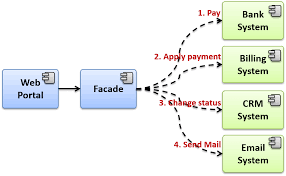
\includegraphics[width=10cm]{./images/1} 
	\end{center}

	
	\begin{center}
	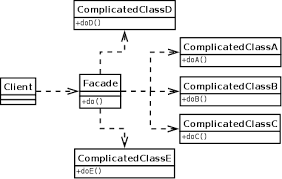
\includegraphics[width=10cm]{./images/2} 
	\end{center}


Busca simplificar el sistema, desde el punto de vista del cliente, proporcionando una interfaz unificada para un conjunto de subsistemas, definiendo una interfaz de nivel más alto. Esto hace que el sistema sea más fácil de usar.

Este patrón busca reducir al mínimo la comunicación y dependencias entre subsistemas. Para ello, utilizaremos una fachada, simplificando la complejidad al cliente. El cliente debería acceder a un subsistema a través del Facade. De esta manera, se estructura un entorno de programación más sencillo, al menos desde el punto de vista del cliente (por ello se llama "fachada").


         \item ¿Se debe utilizar cuando?
	\\ Se quiera proporcionar una interfaz sencilla para un subsistema complejo.
             Se quiera desacoplar un subsistema de sus clientes y de otros subsistemas, haciéndolo más independiente y portable.
            Se quiera dividir los sistemas en niveles: las fachadas serían el punto de entrada a cada nivel. Facade puede ser utilizado a nivel aplicación.
	\begin{center}
	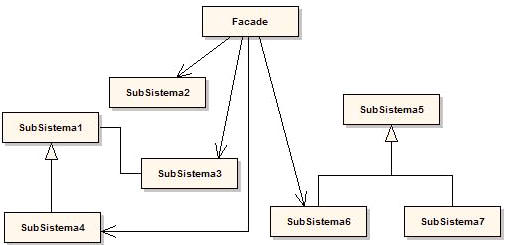
\includegraphics[width=10cm]{./images/3} 
	\end{center}

Los clientes se comunican con el subsistema a través de la facade, que reenvía las peticiones a los objetos del subsistema apropiados y puede realizar también algún trabajo de traducción. Los clientes que usan la facade no necesitan acceder directamente a los objetos del sistema.	
	

\end{itemize} 


\end{flushleft}
\section{ Conclusiones y Trabajos Futuros} 
\textbf{........................................}\\
\begin{flushleft}
......................................
\end{flushleft}
\section{ Patrones de Diseño:Especificación de la Capa de Aplicación} 
\textbf{........................................}\\
\begin{flushleft}
......................................
\end{flushleft}


\end{document}